\section{Interest Rate Differentials as Differences in Risk Premia}

\begin{figure}[htp!]
  \centering
  \caption{New Zealand Dollar - Japanese Yen Exchange Rate}
  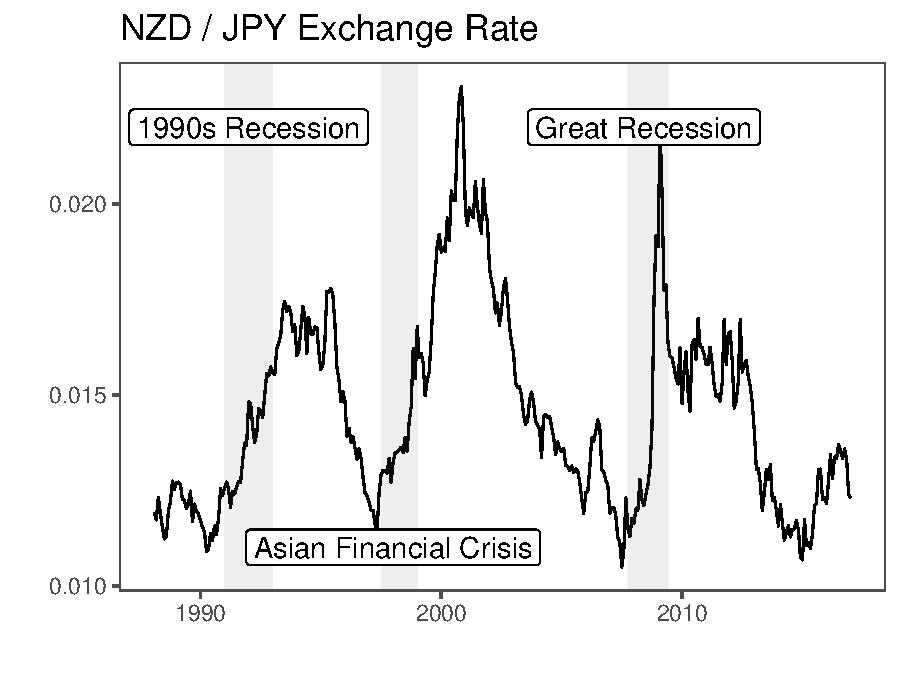
\includegraphics[width=0.7\textwidth]{Exhibits/Figure_FX_JPYNZD.pdf}
  \label{fig:spot}
\end{figure}
Continuing with our example from Figure \ref{fig:fp}, Figure
\ref{fig:spot} plots the New Zealand dollar - Japanese yen exchange
rate in terms of dollars per yen. An increase in the exchange rate
indicates yen appreciation. The shaded areas highlight three distinct
periods of global economic turmoil: The early 1990s recession (1990 -
1993), the Asian financial crisis (1997 - 1998), and the Great
Recession (2007 - 2009). In each of these periods, the yen appreciated
markedly against the New Zealand Dollar. If these appreciations during
periods of economic turmoil are part of a broader pattern, investors
should naturally consider the Japanese yen the safer currency. Hence,
the lower returns earned on Japanese yen investments may be a result
of the yen's usefulness as a hedge against bad times. On the other
hand, we should expect investing in the New Zealand dollar earns
higher returns, because the New Zealand dollar provides none of the
hedging benefits of the Japanese yen and is therefore a riskier
currency for global investors.

\subsection{Reduced-form Evidence}

To formally attribute the returns of currency traders to risk, we need
to borrow some technology from the broader asset pricing literature.
A large empirical asset pricing literature constructs
\emph{risk-factors} to attribute cross-sectional differences in asset
returns to different sources of risk by looking for comovement in
asset returns \citep{Fama1976}. Typically, researchers sort assets
based on some characteristic of interest, and then divides asset into
a small number of portfolios based on the sort. The first portfolio
typically contains assets with the lowest values of the characteristic
of interest, and the last portfolio typically contains assets with the
highest values. A risk factor is then constructed by taking the
difference in returns between the fist and last portfolio. Researchers
determine a risk factor explains asset returns by running regressions
of returns on the risk factor, and showing that assets with higher
regression coefficients on the risk factor also obtain higher expected
returns.\footnote{For example, \citet{FamaFrench1992} constructed two
  risk factors by sorting U.S. equities into portfolios based on
  market capitalization and book-to-market ratio, and showed
  portfolios of stocks with greater exposure to these two risk factors
  obtained higher average returns.}

% A key innovation of the empirical asset pricing literature is also
% to analyze portfolio returns rather returns than on individual
% assets. Again, assets are sorted into portfolios based on some
% dimension of interest. Intuitively, averaging the returns of assets
% within portfolios eliminates diversifiable and asset-specific risks.
% The remaining variation in returns across portfolios should better
% capture the risk-return trade-off specifically from differing along
% the dimension of interest.

In a seminal paper, \citet{LustigRoussanovVerdelhan2011} applied these
asset pricing techniques to exchange rates and provided systematic
evidence that the greater returns obtained from investing in
high-interest-rate currencies result from greater risk exposure. For
every month between November 1983 and December 2009, the authors
sorted currencies into 6 portfolios based on their risk-free rate
differential relative to the U.S. dollar. The first portfolio
contained currencies with the lowest risk-free rates and the last
portfolio contained currencies with the highest risk-free rates. The
authors constructed a \emph{carry trade} risk factor by taking the
difference in the returns between the portfolio containing the
highest-interest-rate currencies and the portfolio containing the
lowest-interest-rate currencies.

\citet{LustigRoussanovVerdelhan2011} showed that differential exposure
to their carry trade risk factor accounted the expected returns from
investing in different currencies. The authors regressed the returns
of their 6 currency portfolios on their carry trade risk factor. The
portfolios with higher-interest-rate currencies obtained a higher
average return and also covaried more positively with the risk factor.
An increase in the regression coefficient on the carry trade risk
factor from 0 to 1 was associated with a large and highly significant
increase of 5.5 percent per year.

In this sense, \citet{LustigRoussanovVerdelhan2011} identified a
common source of risk in currency markets, and showed that exposure to
this common source of risk explained cross-sectional differences in
currency returns. However, the major drawback of this asset pricing
method is that it does not reveal the ultimate source of risk. In
other words, we know exchange rates move with each other, but we do
not know the economic forces that drive this comovement.

Hence, many researchers have tried to identify relationships between
currency returns and macro-financial variables to understand the
source of currency risk. \citet{LustigVerdelhan2007} showed that
low-interest-rate currencies provide a hedge against U.S. consumption
growth risk. Low-interest-rate currencies systematically appreciate
when U.S. consumption growth is low, and high-interest-rate currencies
tend to depreciate when U.S. consumption growth is low. Thus, the U.S.
investor can hedge against periods of low consumption growth by
investing in a portfolio of low-interest-rate currencies. U.S.
investors find this hedging property useful, and therefore accept a
lower rate of return.

Moreover, low-interest-rate currencies tend to appreciate during
periods of financial turmoil, whereas high-interest-rate currencies
tend to depreciate. \citet{LustigRoussanovVerdelhan2011} and
\citet{CampbellMedeirosViceira2010} showed low-interest-rate
currencies tend to appreciate whenever equity markets are volatile.
Consistent with this evidence, \citet{Menkhoffetal2012} measure of
periods financial market turmoil using exchange rate data, and show
low-interest-rate currencies provide a hedge against periods of high
exchange rate volatility.

Literature on crash risk:
\begin{itemize}
\item \citet{Brunnermeieretal2009} studied eight major currencies.
  Higher interest rate currencies exhibited greater chance of large
  devaluations (i.e. crash risk).
\item Jurek2014 - Constructs carry trades without crash risk to
  quantify the contribution of crash risk to carry trades. At most
  1/3.
\item Farhietal2015 - Similar to Jurek. How much of the carry trade is
  driven by crash risk? Also arrives at around 1/3.
\item Lewis2011 - peso problems (no risk premia, simply mismeasuring
  average returns due to small samples)
\end{itemize}

Each of these papers highlight different ways in which
high-interest-rate currencies may be riskier than low-interest-rate
currencies. However, the common thread among these papers is that the
persistent differences in returns to investing in various currencies
reflect persistent differences in the stochastic properties of their
exchange rates. Under this interpretation, currencies yielding lower
returns are safer currencies that tend to appreciate during periods of
economic distress.